\definecolor{chNineteenTaskBlue}{RGB}{46,84,151}
\begin{tikzpicture}[x=0.110mm,y=-0.110mm]
  \node[anchor=north west,inner sep=0] at (0,0) {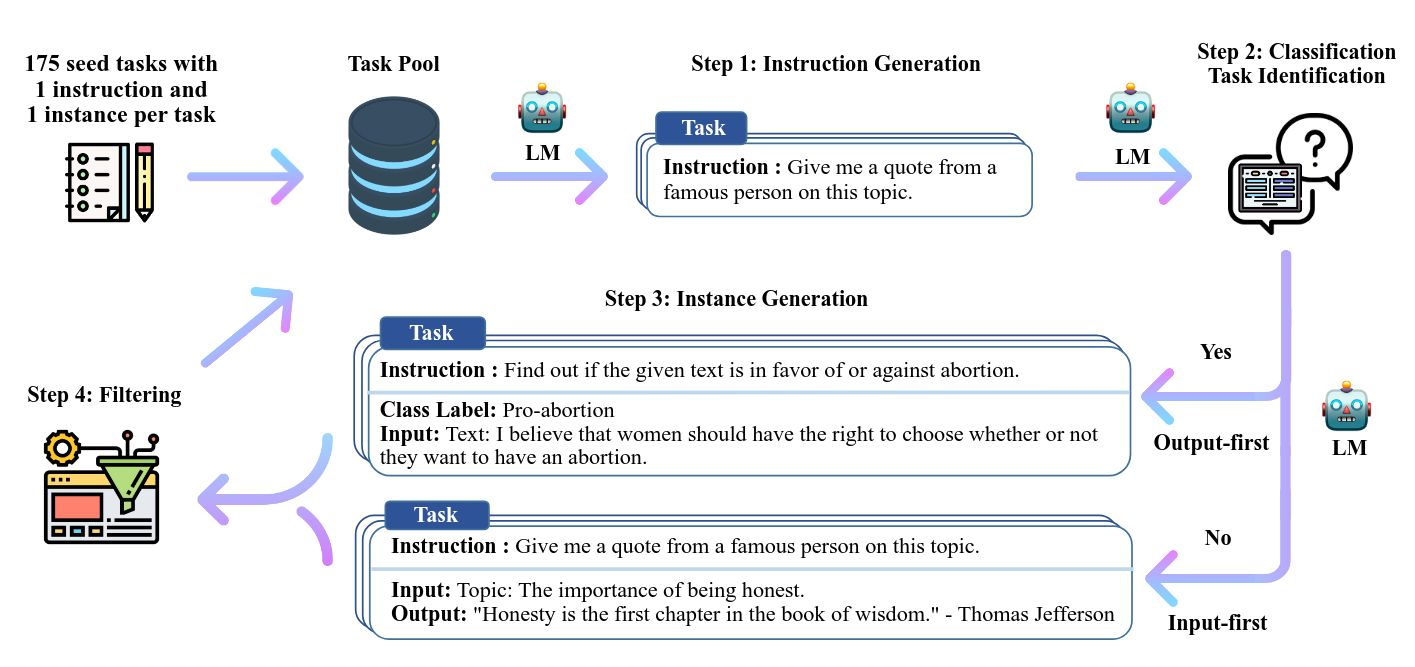
\includegraphics[width=155.65mm]{part6/visuals/self-instruct.png}};
  \fill[white] (16,43) rectangle (245,125);
  \node[align=center,font=\fontsize{8}{9.2}\selectfont] at (129,84) {175 项种子任务\\每项含 1 条指令\\和 1 个实例};
  \fill[white] (342,47) rectangle (457,79);
  \node[font=\footnotesize\bfseries] at (397,63) {任务池};
  \fill[white] (680,42) rectangle (1001,83);
  \node[font=\footnotesize\bfseries] at (838,64) {步骤 1：指令生成};
  \fill[white] (518,139) rectangle (566,165);
  \node[font=\fontsize{7.3}{8}\selectfont] at (542,151) {语言模型};
  \fill[chNineteenTaskBlue] (657,114) rectangle (746,141);
  \node[text=white,font=\fontsize{7.5}{8.5}\selectfont\bfseries] at (702,127) {任务};
  \fill[white] (660,151) rectangle (1027,205);
  \node[anchor=north west,text width=38.8mm,align=left,font=\fontsize{7.5}{8.5}\selectfont,inner sep=0pt] at (664,156) {\textbf{指令：}给我一句有关这一主题的名人名言。};
  \fill[white] (1184,36) rectangle (1413,89);
  \node[align=center,font=\fontsize{8}{9.5}\selectfont\bfseries] at (1294,63) {步骤 2：识别\\分类任务};
  \fill[white] (1109,143) rectangle (1155,168);
  \node[font=\fontsize{7.3}{8}\selectfont] at (1132,155) {语言模型};
  \fill[white] (593,281) rectangle (877,313);
  \node[font=\footnotesize\bfseries] at (736,299) {步骤 3：实例生成};
  \fill[chNineteenTaskBlue] (383,319) rectangle (484,346);
  \node[text=white,font=\fontsize{7.5}{8.5}\selectfont\bfseries] at (433,333) {任务};
  \fill[white] (376,355) rectangle (1123,388);
  \node[anchor=west,font=\fontsize{8}{9}\selectfont,inner sep=0pt] at (380,373) {\textbf{指令：}判断给定文本支持还是反对堕胎。};
  \fill[white] (375,395) rectangle (1123,467);
  \node[anchor=north west,text width=80mm,align=left,font=\fontsize{8}{9.2}\selectfont,inner sep=0pt] at (380,400) {\textbf{类别标签：}支持堕胎\\\textbf{输入：}文本：我认为，女性应有权选择自己是否要堕胎。};
  \fill[white] (1185,335) rectangle (1260,365);
  \node[font=\fontsize{8}{9}\selectfont\bfseries] at (1223,351) {是};
  \fill[white] (1147,426) rectangle (1283,460);
  \node[font=\fontsize{8}{9}\selectfont\bfseries] at (1215,443) {输出优先};
  \fill[white] (1325,433) rectangle (1380,461);
  \node[font=\fontsize{7.3}{8}\selectfont] at (1353,448) {语言模型};
  \fill[chNineteenTaskBlue] (386,503) rectangle (487,529);
  \node[text=white,font=\fontsize{7.5}{8.5}\selectfont\bfseries] at (436,516) {任务};
  \fill[white] (374,532) rectangle (1126,566);
  \node[anchor=west,font=\fontsize{8}{9}\selectfont,inner sep=0pt] at (380,548) {\textbf{指令：}给我一句有关这一主题的名人名言。};
  \fill[white] (374,575) rectangle (1124,631);
  \node[anchor=west,font=\fontsize{7.5}{8.5}\selectfont,inner sep=0pt] at (380,589) {\textbf{输入：}主题：诚实的重要性。};
  \node[anchor=west,font=\fontsize{7.5}{8.5}\selectfont,inner sep=0pt] at (380,615) {\textbf{输出：}“诚实是智慧之书的第一章。”——Thomas Jefferson};
  \fill[white] (1194,521) rectangle (1256,551);
  \node[font=\fontsize{8}{9}\selectfont\bfseries] at (1224,537) {否};
  \fill[white] (1157,605) rectangle (1289,639);
  \node[font=\fontsize{8}{9}\selectfont\bfseries] at (1222,622) {输入优先};
  \fill[white] (14,376) rectangle (202,412);
  \node[font=\fontsize{8}{9}\selectfont\bfseries] at (105,395) {步骤 4：过滤};
\end{tikzpicture}
